% -*- TeX:de -*-
\NeedsTeXFormat{LaTeX2e}
\documentclass[12pt,a4paper]{article}
\usepackage[german]{babel} % german text
\usepackage[DIV12]{typearea} % size of printable area
\usepackage[T1]{fontenc} % font encoding
%\usepackage[latin1]{inputenc} % most likely on Windows
\usepackage[utf8]{inputenc} % probably on Linux
\usepackage{multicol}

% PLOTTING
\usepackage{pgfplots} 
\usepackage{pgfplotstable}
\usepackage{url}
\usepackage{graphicx} % to include images
\usepackage{tikz}
\usepackage{subfigure} % for creating subfigures
\usepackage{amsmath} % a bunch of symbols
\usepackage{amssymb} % even more symbols
\usepackage{booktabs} % pretty tables
\usepackage{makecell} % multi row table heading

% a floating environment for circuits
\usepackage{float}
\usepackage{caption}

%\newfloat{circuit}{tbph}{circuits}
%\floatname{circuit}{Schaltplan}

% a floating environment for diagrams
%\newfloat{diagram}{tbph}{diagrams}
%\floatname{diagram}{Diagramm}

\selectlanguage{german} % use german

\begin{document}

%%%%%%% DECKBLATT %%%%%%%
\thispagestyle{empty}
			\begin{center}
			\Large{Fakultät für Physik}\\
			\end{center}
\begin{verbatim}


\end{verbatim}
							%Eintrag des Wintersemesters
			\begin{center}
			\textbf{\LARGE WS 2013/14}
			\end{center}
\begin{verbatim}


\end{verbatim}
			\begin{center}
			\textbf{\LARGE{Physikalisches Praktikum\\ für das Bachelorstudium}}
			\end{center}
\begin{verbatim}




\end{verbatim}

			\begin{center}
			\textbf{\LARGE{PROTOKOLL}}
			\end{center}
			
\begin{verbatim}

\end{verbatim}

			\begin{flushleft}
			\textbf{\Large{Experiment (Nr., Titel):}}\\
							%Experiment Nr. und Titel statt den Punkten eintragen
			\LARGE{PW10 Wechselstrom I}	
			\end{flushleft}

\begin{verbatim}

\end{verbatim}	
							%Eintragen des Abgabedatums, oder des Erstelldatums des Protokolls
			\begin{flushleft}
			\textbf{\Large{Datum:}} \Large{21.11.2013}
			\end{flushleft}
			
\begin{verbatim}
\end{verbatim}
							%Namen der Protokollschreiber
		\begin{flushleft}
			\textbf{\Large{Namen:}} \Large{Patrick Braun, Johannes Kurz}
			\end{flushleft}

\begin{verbatim}


\end{verbatim}
							%Kurstag und Gruppennummer, zb. Fr/5
			\begin{flushleft}
			\textbf{\Large{Kurstag/Gruppe:}} \Large{DO/2}
			\end{flushleft}

\begin{verbatim}

\end{verbatim}
							%Name des Betreuers, das Praktikum betreute.
			\begin{flushleft}
			\LARGE{\textbf{Betreuer:}}	\Large{Wilhelm Markowitsch}	
			\end{flushleft}

%%%%%%% DECKBLATT ENDE %%%%%%%
\pagebreak
\setlength{\columnsep}{20pt}
\begin{multicols}{2}

%%%%%%%%%%%%%%%%%%%%%%%%%%%%%%%%%%%%%%%%%%%%%%%%

%\begin{figure}[H]
%	\centering
%	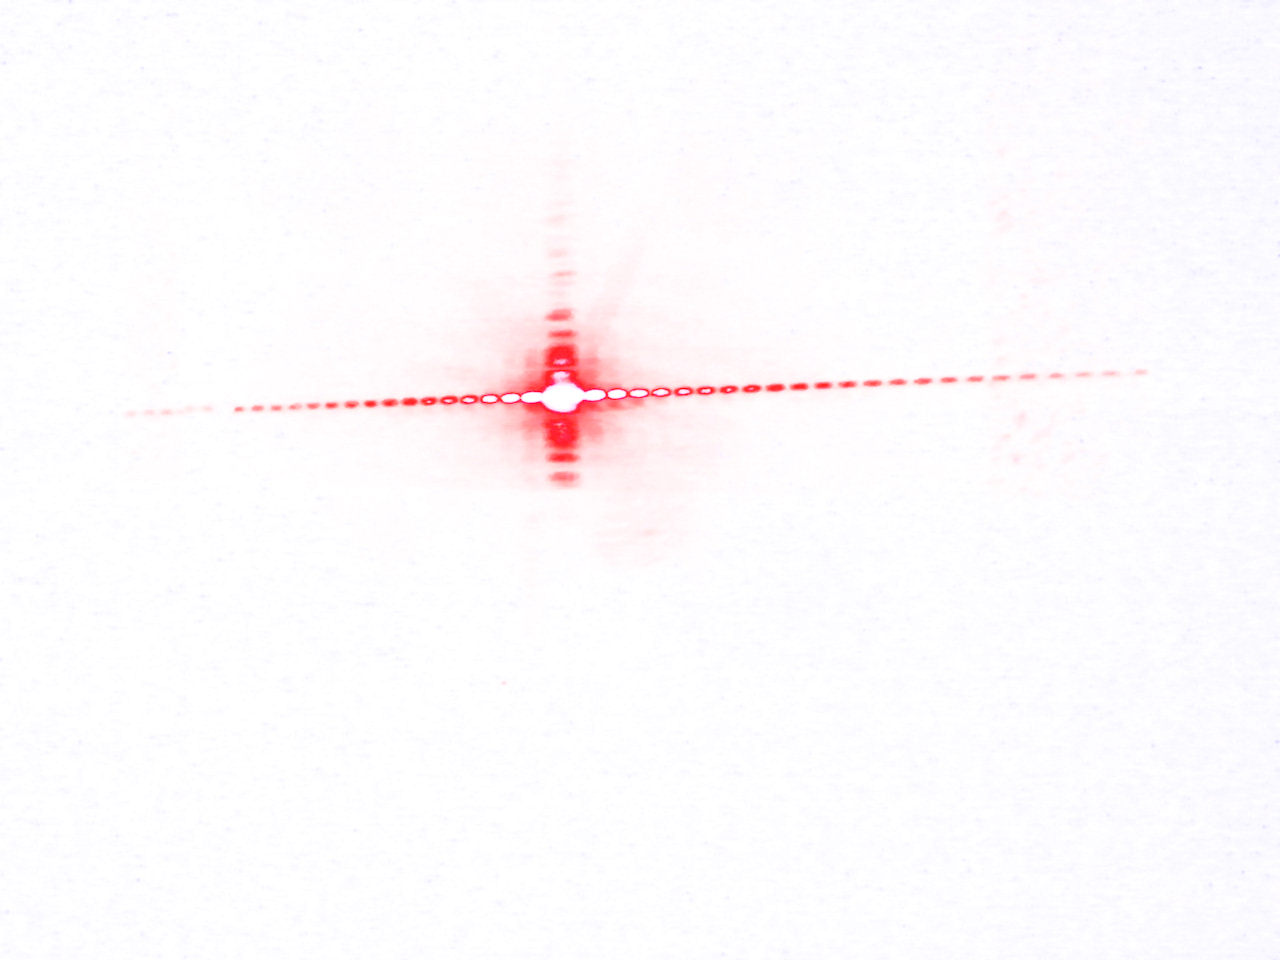
\includegraphics[scale=0.35]{./figure/beugung.png}
%	\caption{Beugungsmuster Einzelspalt (echtes Foto; schwarz durch weiß ersetzt)}
%	\label{fig:beugungsmuster}
%\end{figure}


%\begin{figure}[H]
%	\centering
%	\pgfplotstabletypeset[
%			columns={abstand, n},
%			col sep=&,
%			columns/abstand/.style={precision=2, zerofill, column name=\makecell{$Abstand$\\$(\pm 0.05)[mm]$} }, 
%			columns/n/.style={column name=\makecell{$n$\\$(Ordnung)$}, precision=0},
%			every head row/.style={before row=\hline,after row=\hline\hline},
%			every last row/.style={after row=\hline},
%			every first column/.style={column type/.add={|}{} },
%			every last column/.style={column type/.add={}{|} }
%			]{
%			abstand & n
%			12.9 & 1
%			24.45 & 2
%			37.40 & 3
%			49.35& 4
%			62.45 & 5
%			74.45 & 6
%			87.45 & 7
%			100.25 & 8
%			
%			}
%	\caption{Messwerte Einzelspalt}
%	\label{tab:werte_einzelspalt}
%\end{figure}
%


\section{Temperaturabhängigkeit des elektrischen Widerstandes}

Im ersten Teil von PW10 sollen die Widerstände 3er verschiedener Stoffe in Abhängigkeit der Temperatur bestimmt werden: Ein \textbf{Kaltleiter (PTC)}, ein  \textbf{Heißleiter (NTC)} und ein  \textbf{Elektrolyt}.
\\
Im Allgemeinen hängt der Widerstand (oder eben die Leitfähigkeit) eines Materials von der Zahl der freien Ladungsträger und deren Beweglichkeit ab. In PTC und NTC (also den Feststoffen) dienen als Ladungstäger die Elektronen im Leitungsband. Das ist derjenige Energie-Bereich, der über dem Valenzband liegt, dem höchsten, von Elektronen annähernd voll besetzten, Bereich.\\
\\
In Kaltleitern gehen diese Energieniveau-Bereiche ineinander über. Daher liegt der Grundzustand vieler Elektronen schon im Leitungsband. Steigt jedoch die Temperatur, schwingen die Atome stärker und behindern so die Bewegung der Elektronen. Der Widerstand steigt also mit steigender Temperatur.
\\
Dieser Effekt tritt auch bei Halbleitern (Heißleiter, NTC) auf, ist aber verschwindend gering, im Vergleich zur Steigerung der Leitfähigkeit mit zunehmender Temperatur: Die Elektronen in Halbleitern müssen eine gewisse Energielücke überwinden um vom Valenz- ins Leitungsband zu kommen. Steigt also die thermische Energie, steigt auch die Leitfähigkeit (exponentiell) an.
\\
In Fluiden können, im Gegensatz zu Feststoffen, Ionen oder sogar Moleküle Ladungsträger sein. Ihre Beweglichkeit hängt von der Viskosität ab. Diese nimmt exponentiell ab mit der Temperatur ab.
\\
Der Widerstand des Elektrolyts und des Halbleiters zeigen also eine ähnliche Temperaturabhängigkeit, wenn auch aus völlig verschiedenen Gründen.
\\
\begin{figure}[H]
	\centering
	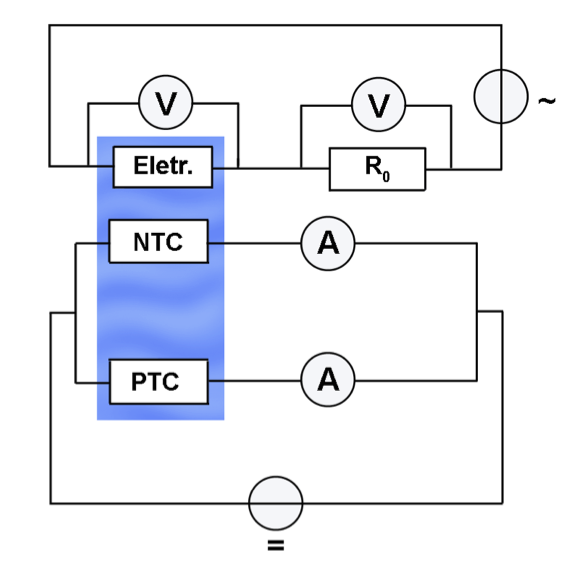
\includegraphics[scale=0.80]{./figure/schaltskizze_temp-widerst.png}
	\caption{Schaltskizze des Messaufbaus mit allen 3 Widerständen}
	\label{fig:schaltskizze_temp-widerst}
\end{figure}

Im Aufbau befinden sich alle 3 Widerstände in einem beheizbaren Wasserbad (destilliertes Wasser), mit einem Rührer, um die Temperatur des Wassers so gleichmäßig verteilt, wie möglich, zu halten.\\
NTC und PTC sind, in Parallelschaltung,  an eine 2V Gleichstrom-Spannungsquelle angeschlossen. An beiden Zweigen wird der Strom gemessen, durch den, mithilfe der konstanten Spannung, der Widerstand berechnet werden kann.\\
Mit dem Elektrolyt in Serie ist ein bekannter Widerstand $R_0$ geschaltet. An beiden wird die jeweils anliegende Spannung gemessen. Der Stromkreis wird mit 8V Wechselstrom betrieben.\\
Außerdem wird die Temperatur im Wasserbad gemessen.\\
Alle Messungen werden mit Cassy-Lab-Sensoren durchgeführt. Zuerst wird das Wasserbad auf etwa $80^\circ C$ erhitzt. Während dem Abkühlen werden die Messungen automatisch (2 Messungen/Minute) durchgeführt.\\
\\
\begin{itemize}
	\item \textbf{Elektrolyt}
	Die gemessenen Widerstände werden gegen die Temperatur aufgetragen. Durch einen Exponentialfit der Daten soll gezeigt werden, dass die exponentielle Beziehung tatsächlich gilt.\\
	Dabei soll in diesem Praktikumsbeispiel nicht näher auf die Viskosität eingegangen werden.
	
	\item \textbf{Halbleiter}
	Der Widerstand ist gegeben durch
	$$R(T)=R_{T_0}e^{-b\cdot (\frac{1}{T_0}- \frac{1}{T})}$$
	Durch Umformung erhalten wir die Geradengleichung:
	$$ln{\frac{R(T)}{R_{T_0}}}=b\cdot \frac{1}{T} + d$$
	wobei $R_{T_0}$ und $d$ miteinander in Beziehung stehen und hier nicht von Bedeutung sind.\\
	Die Lückenenergie $E_g$ des Halbleiters lässt sich aus dem Temperaturkoeffizienten $b$ berechnen:
	$$E_g = b \cdot 2k_B$$
	Von $E_g$ soll auf das verwendete Material geschlossen werden.
	
	\item \textbf{Kaltleiter}
	$$R(T) = R_{T_0} * [1+ \alpha (T - T_0)]$$
	$R(T)$ wird gegen $(T-T_0)$ aufgetragen ($T_0$ wird $20^\circ C$ gesetzt um mit der gegebenen Tabelle vergleichen zu können). \\
	Der y-Achsenabschnitt gibt $R_{T_0}$ und indem die Steigung der Gerade durch $R_{T_0}$ geteilt wird, erhalten wir den Temperaturkoeffizienten $\alpha_{20}$ für $20^\circ C$.\\
	Durch Vergleich soll der verwendete Leiter identifiziert werden.\\
	\\
		
\end{itemize}

\end{multicols}
\begin{figure}[H]
	\centering
	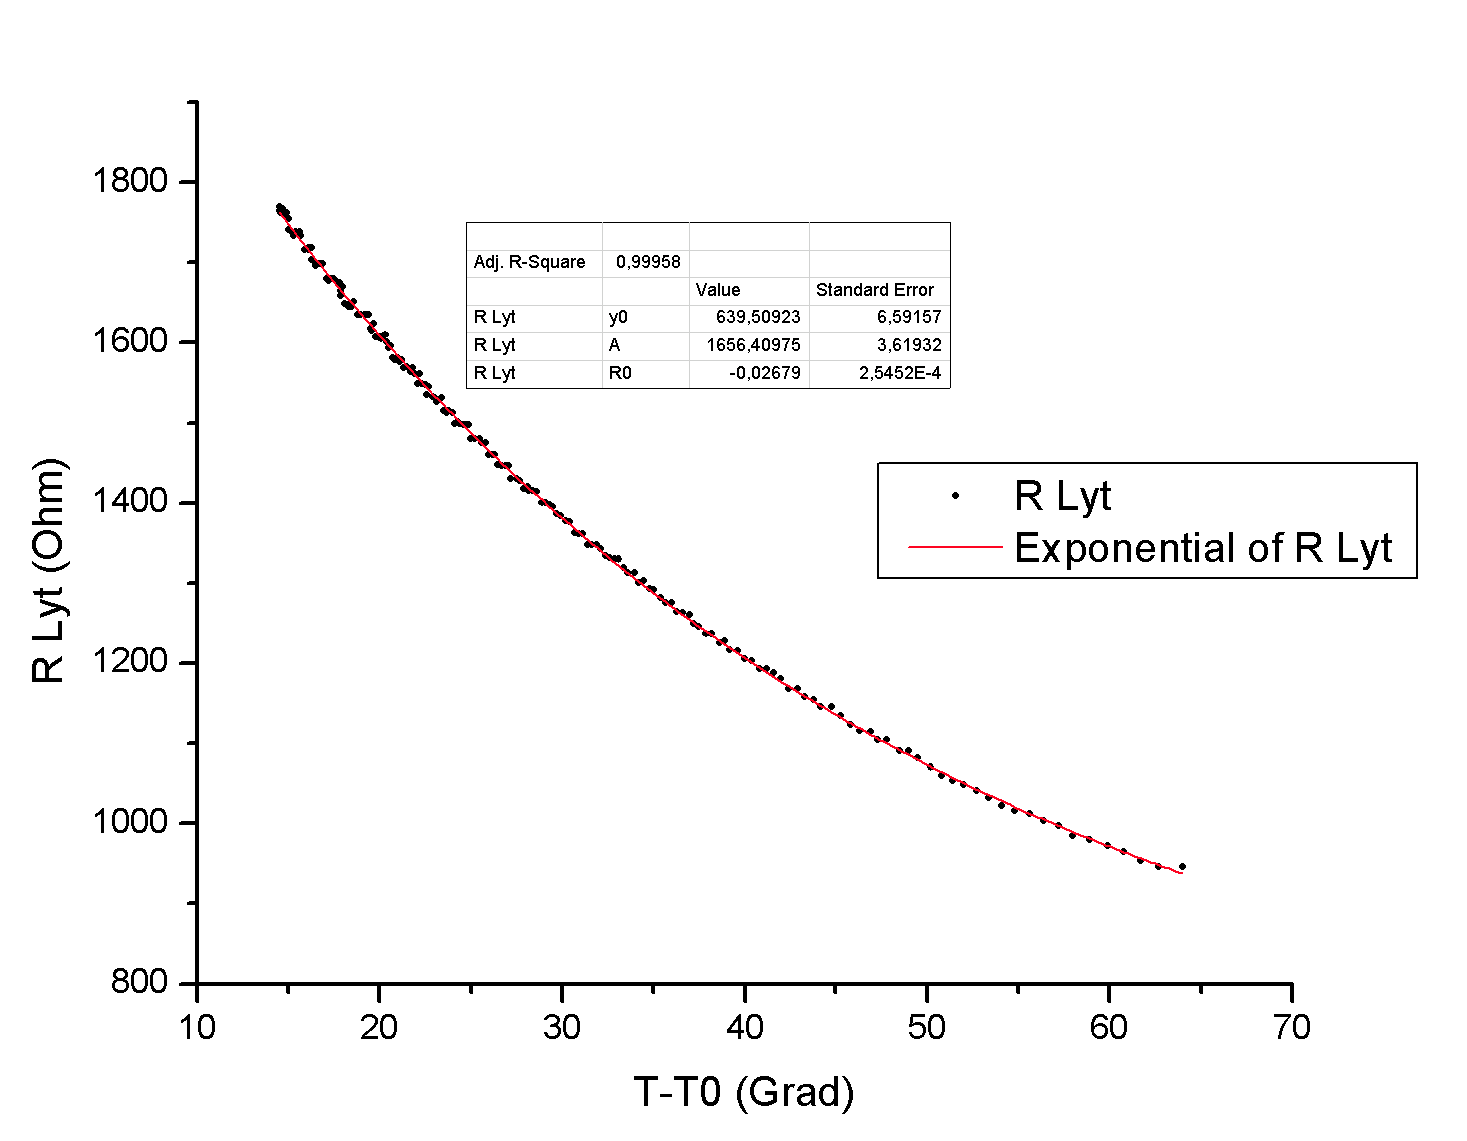
\includegraphics[scale=0.60]{./figure/Rlyt_t_t0.png}
	\caption{Widerstand Elektrolyt mit Exponentiellem Fit}
	\label{fig:rlyt}
\end{figure}
\begin{multicols}{2}

\end{multicols}
\begin{figure}[H]
	\centering
	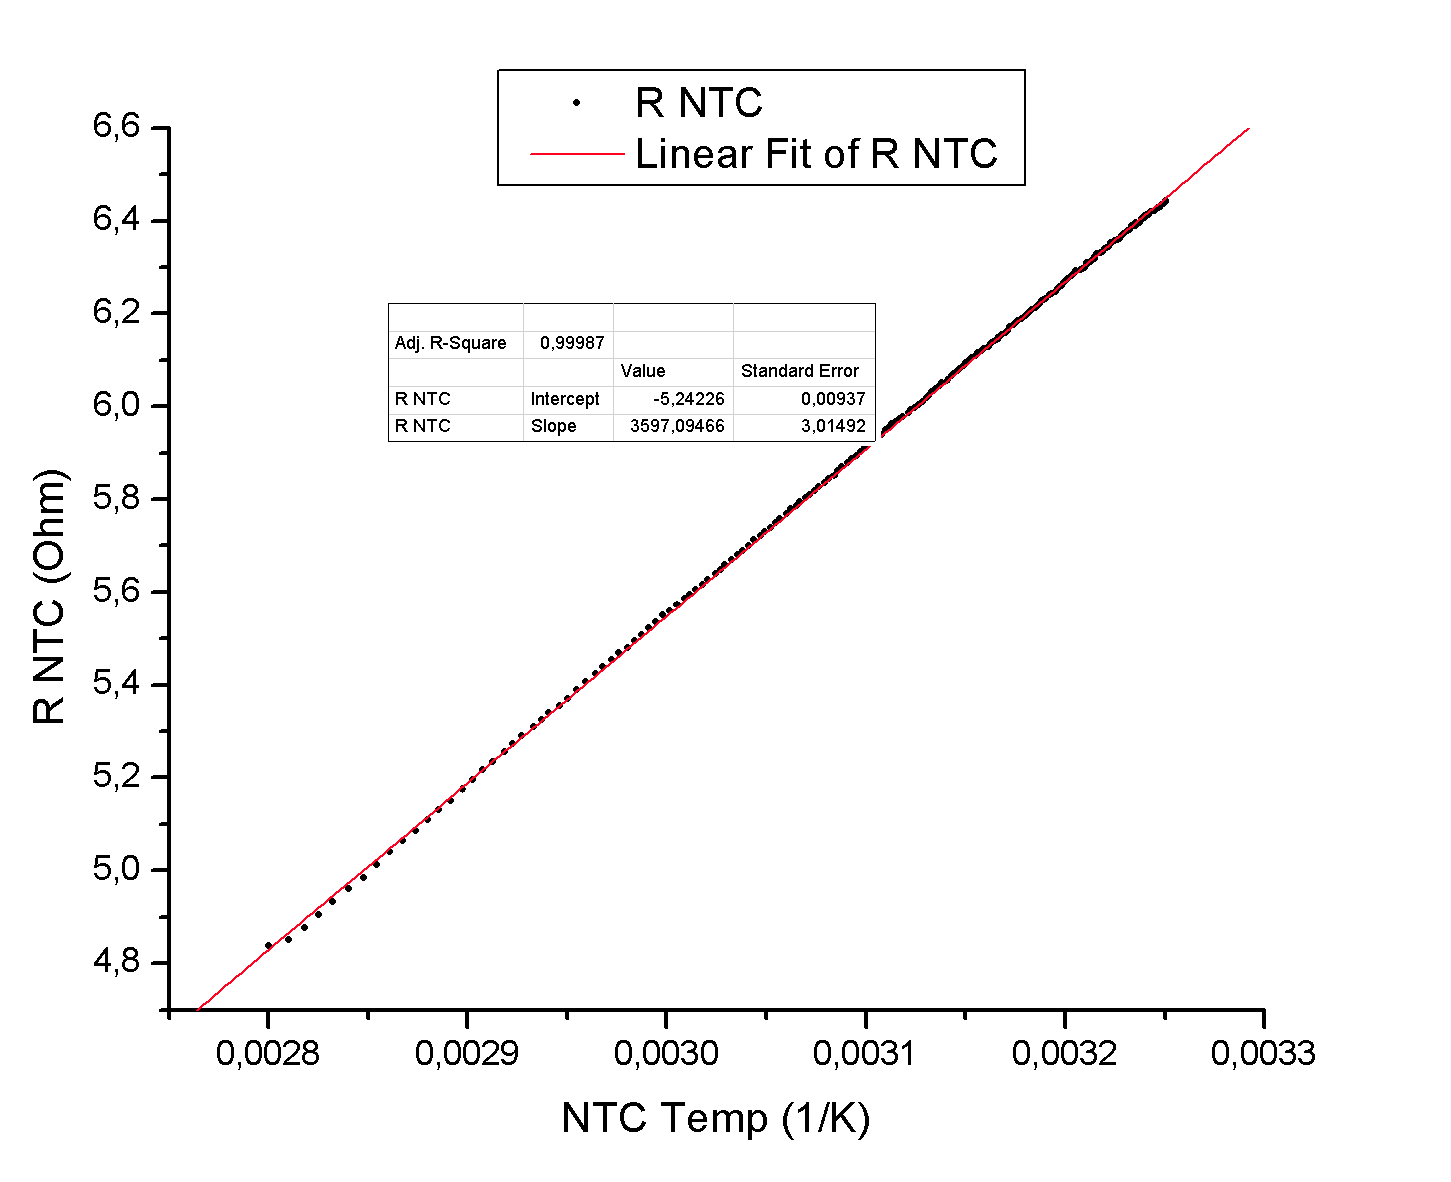
\includegraphics[scale=0.60]{./figure/RNTC_NTC_temp.png}
	\caption{Halbleiter Widerstand mit linearem Fit}
	\label{fig:rntc}
\end{figure}
\begin{multicols}{2}

\end{multicols}
\begin{figure}[H]
	\centering
	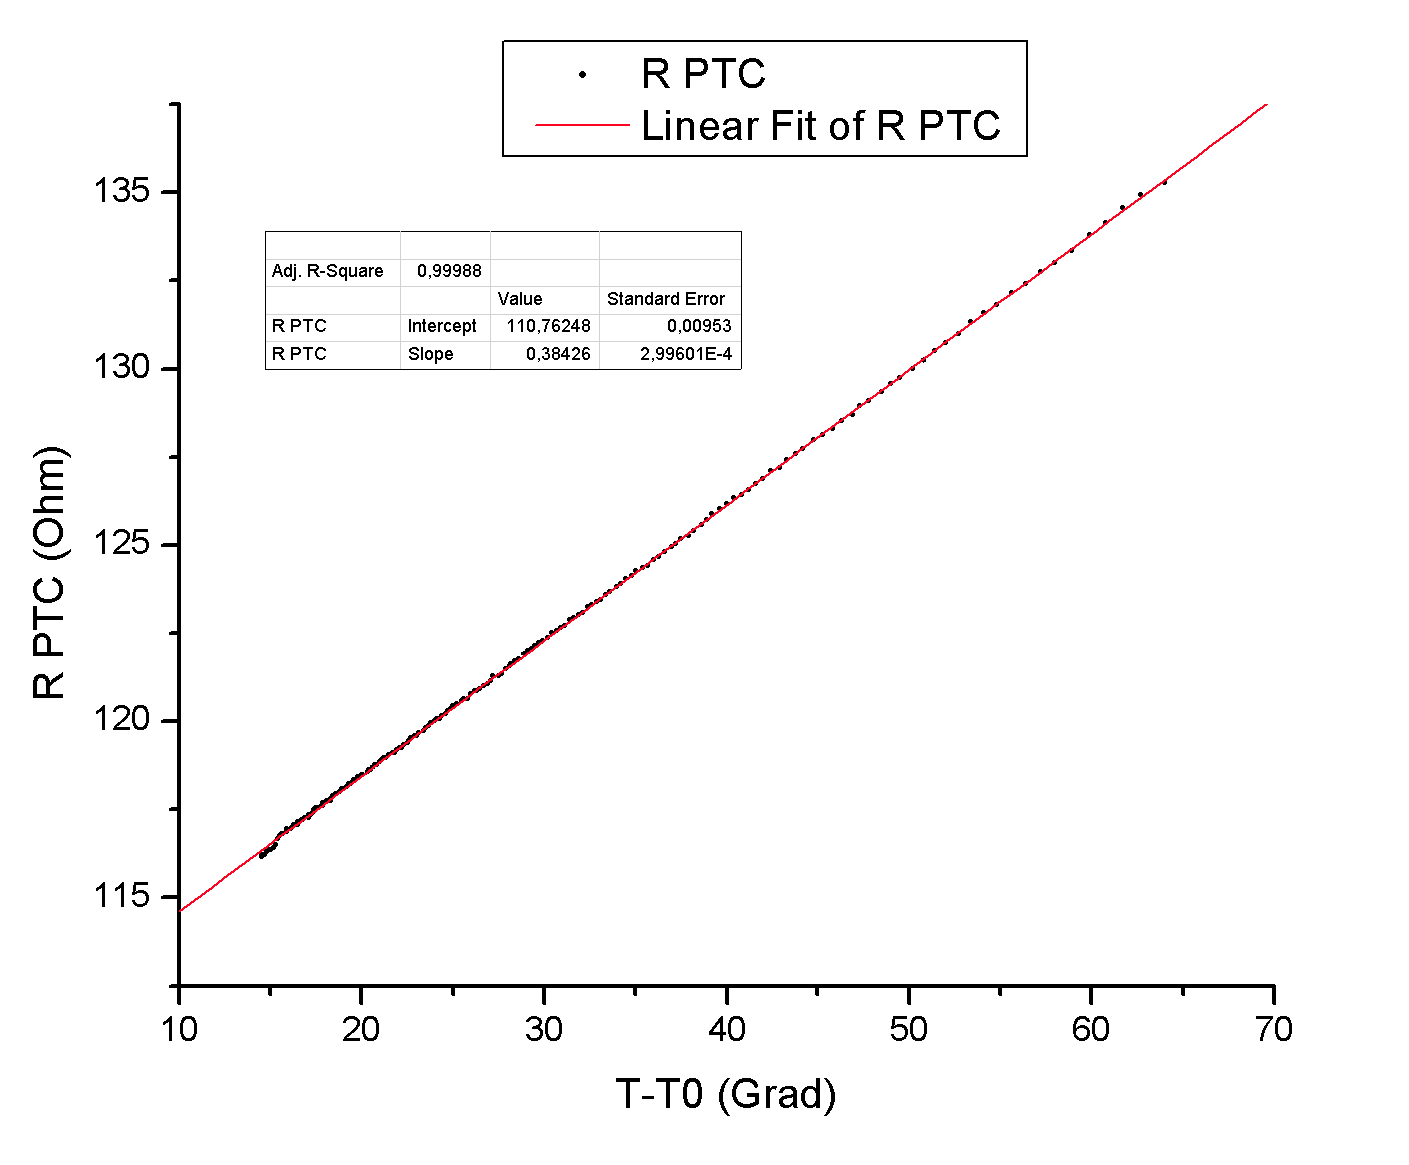
\includegraphics[scale=0.60]{./figure/RPTC_t_t0.png}
	\caption{Metal Widerstand mit linearem Fit}
	\label{fig:rptc}
\end{figure}
\begin{multicols}{2}

\subsection{Messwerte und Ergebnisse}
$U_{=} = (2.063 \pm 0.004)V$\\
\indent Gleichspannung (NTC \& PTC):\\
$T_0 = 20^\circ C$ gesetzt\\

%%%TO DO %%%%%%
%Graphen importieren
%Graphen indizieren und referenzieren
%unsicherheit aus der regression entnehmen
%fehlerrechnung:

%Kaltleiter:
% delta_alpha= alpha*SQRT((delta R_T0 / R_T0)^2+(delta Steigung/ Steigung)^2)


%Halbleiter:
% delta E_g = deltab * 2* boltzmanconstant


\noindent \textbf{Kaltleiter (PTC)}


%$$ \alpha_{20} = (3400 \pm       )K^{-1}$$
% $$R_{T_0=20} = (110.76 \pm    )\Omega$$
Vermutung: Platin

\noindent \textbf{Halbleiter (NTC)}

% $$b = (3597.04 \pm     )K$$
% $$E_g = (0.6198 \pm    )eV$$
Vermutung: Germanium

\noindent \textbf{Elektrolyt}

%% Kurve mit exp - fit


\subsection{Diskussion}





%%%%%%%%%%%%%%%%%%%%%%%%%%%%%%%%%%%%%%%%%%%%%%%%
\section{Transformator}



\subsection{Messwerte und Ergebnisse}



\subsection{Diskussion}





%%%%%%%%%%%%%%%%%%%%%%%%%%%%%%%%%%%%%%%%%%%%%%%%%%


\section{Quellen}
$[1]$ Leitfaden, \url{http://www.univie.ac.at/anfpra/neu1/pw/pw10/PW10.pdf}\\
$[2]$ 
\end{multicols}


\end{document}